
%(BEGIN_QUESTION)
% Copyright 2006, Tony R. Kuphaldt, released under the Creative Commons Attribution License (v 1.0)
% This means you may do almost anything with this work of mine, so long as you give me proper credit

En {\it Lambert-Beer}-lov knytter absorpsjon av lys i et stoff til banelengden for lysstrålen og konsentrasjonen av det absorberende stoffet:

$$A = abc$$

\noindent
Der,

$A$ = Absorbans

$a$ = Ekstinksjonskoeffisient (en konstant for et gitt stoff og en gitt lysbølgelengde)

$b$ = Banen lyset går gjennom stoffet

$c$ = Konsentrasjon av stoff

\vskip 10pt

Videre knytter Lambert-Beer-loven størrelsen "absorbans" til de målte lysintensitetene inn i og ut av den absorberende prøven:

$$A = \log \left({I_0 \over I}\right)$$

\noindent
Der,

$A$ = Absorbans

$I_0$ = Intensitet til innkommende ("innfallende") lys

$I$ = Intensitet til lys som forlater prøven

\vskip 10pt

$$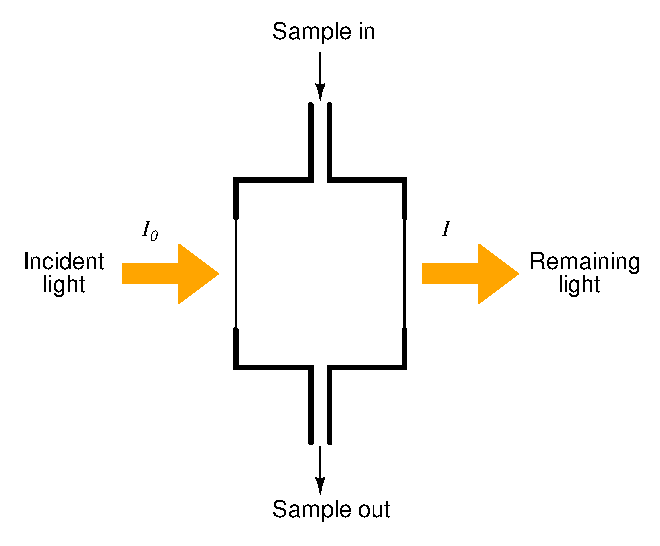
\includegraphics[width=15.5cm]{i00634x01.eps}$$

Basert på én eller begge disse ligningene: bestem om "absorbans" er direkte relatert til et stoffs evne til å dempe en lysstråle, eller om den er omvendt relatert. Med andre ord: har et stoff som demper sterkt liten absorbans eller stor absorbans?

Kombiner deretter ligningene og bruk algebra til å løse for stoffkonsentrasjonen ($c$) gitt målt lysintensitet inn i og ut av en prøve.

\vskip 10pt

Hvis vi vil måle gasskonsentrasjon ved optisk absorpsjon, og vi vet at gassen er en svært svak lysabsorber, hvordan kan vi optimalisere instrumentets følsomhet?

\underbar{file i00634no}
%(END_QUESTION)





%(BEGIN_ANSWER)

Vi kan optimalisere følsomheten ved å maksimere banelengden ($b$).

\vskip 10pt

$$c = {\log \left( {I_0 \over I} \right) \over ab}$$

%(END_ANSWER)





%(BEGIN_NOTES)


%INDEX% Matematikkrepetisjon: manipulere og kombinere ligninger for å danne en ny ligning
%INDEX% Fysikk, optikk: Lambert-Beer-loven

%(END_NOTES)
